\chapname = {MAAS in VENV - II : Controller}

\chapter{\the\chapname}

In this chapter we will discuss the steps required to create a basic MAAS based virtual cloud environment. Remember that the problem statement is to repurpose the commodity hardware to create an experimental cloud. At present we don't have access to those hardwares hence we are conducting our experiments in a virtualized environment. 

\section{Creating an Isolated Network}

MAAS uses DHCP and DNS with PXE boot to enlist the nodes, so naturally you could have a conflict if you deploy this on a network with an existing DHCP server. Hence create a new (virtual) network with the following given steps from the QEMU interface:

\begin{enumerate}
    \setlength\itemsep{0em}
    \item Network name - maasisotest
    \item Disable DHCP configuration
    \item Choose IPv4 address which is not in use by any other connected network. I prefer to use 10.17.17.0/24.
    \item Select forwarding to physical network option and set destination to any physical device and mode to NAT
\end{enumerate}

The network configuration for 'maasisotest' should look similiar to Fig. 4.1. 

\begin{figure}[!ht]
    \centering
    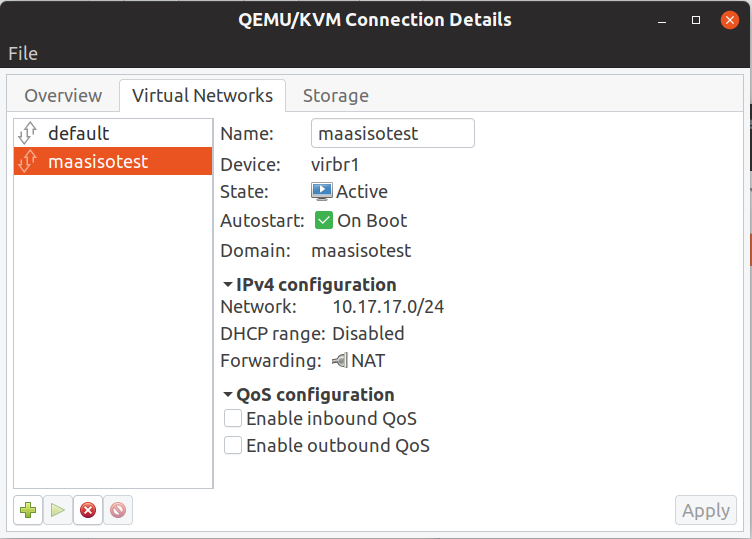
\includegraphics[width=0.5\textwidth]{images/4-1.png}
    \caption{Isolated network configuration}
\end{figure}

This will essentially create a router at the edge of this virtual network.

\section{Creating a maas controller}

Configurations for creating a new virtual machine with ubuntu 18.04 server installation. This machine will act as controller for the maas nodes.

\begin{itemize}
    \setlength\itemsep{0em}
    \item Memory - 1536 MB
    \item CPU Cores - 3
    \item Storage - 20 GB qcow2 
    \item Name - maas-controller
    \item Network - maasisotest
    \item NIC Interface 
    \begin{itemize}
        \item Network source - maasisotest
        \item Device model - virtio
    \end{itemize}
    \item Disk bus - virtio
    \item Remove unnecessary virtual hardware from the list for eg. sound
\end{itemize}

\begin{figure}[!ht]
    \centering
    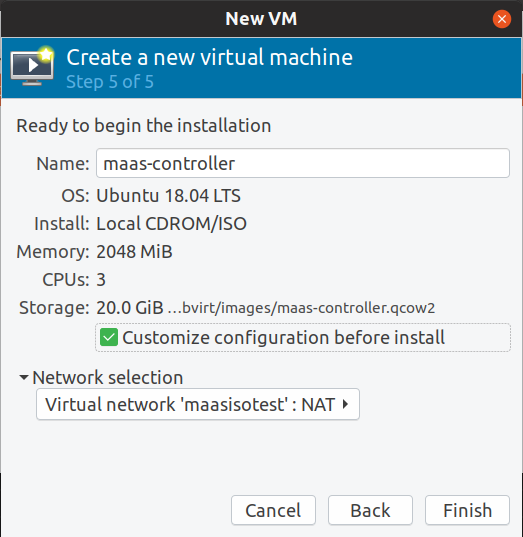
\includegraphics[width=0.5\textwidth]{images/4-2.png}
    \caption{maas-controller configuration}
\end{figure}

The basic configuration for maas-controller should look similar to Fig. 4.2.

Once the configuration is done we can proceed to installation.

\section{Installating ubuntu server image}

During the installation it is expected that DHCP acquisition will fail, since there is no DHCP server on that network. Hence, we need to configure this manually with a statiic IP address.

\begin{figure}[!ht]
    \centering
    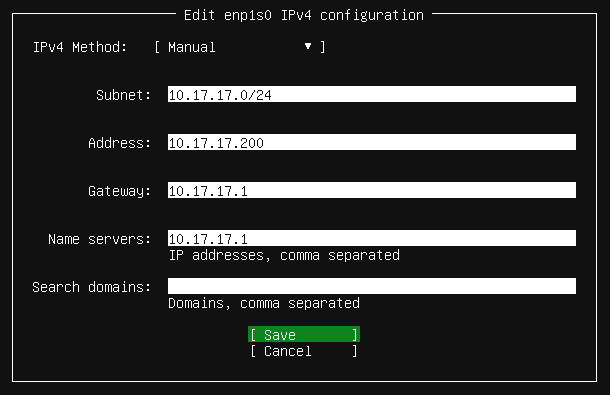
\includegraphics[width=0.5\textwidth]{images/4-3.png}
    \caption{IPv4 configuration}
\end{figure}

Kindly refer to the Fig. 4.3 for the IPv4 configuration.  

Once the installation is finished, the system should reboot.

\section{Setup MAAS}

Use the following commands to install some utility packages and maas related packages on maas-controller. Then verify that you are able to connect through ssh from the host.

\begin{itemize}
    \setlength\itemsep{-1em}
    \item[\$] sudo apt-get install ssh iptraf htop wget lynx dnsutils
    \item[\$] sudo apt-get install maas maas-dhcp maas-dns
\end{itemize}

\begin{figure}[!ht]
    \centering
    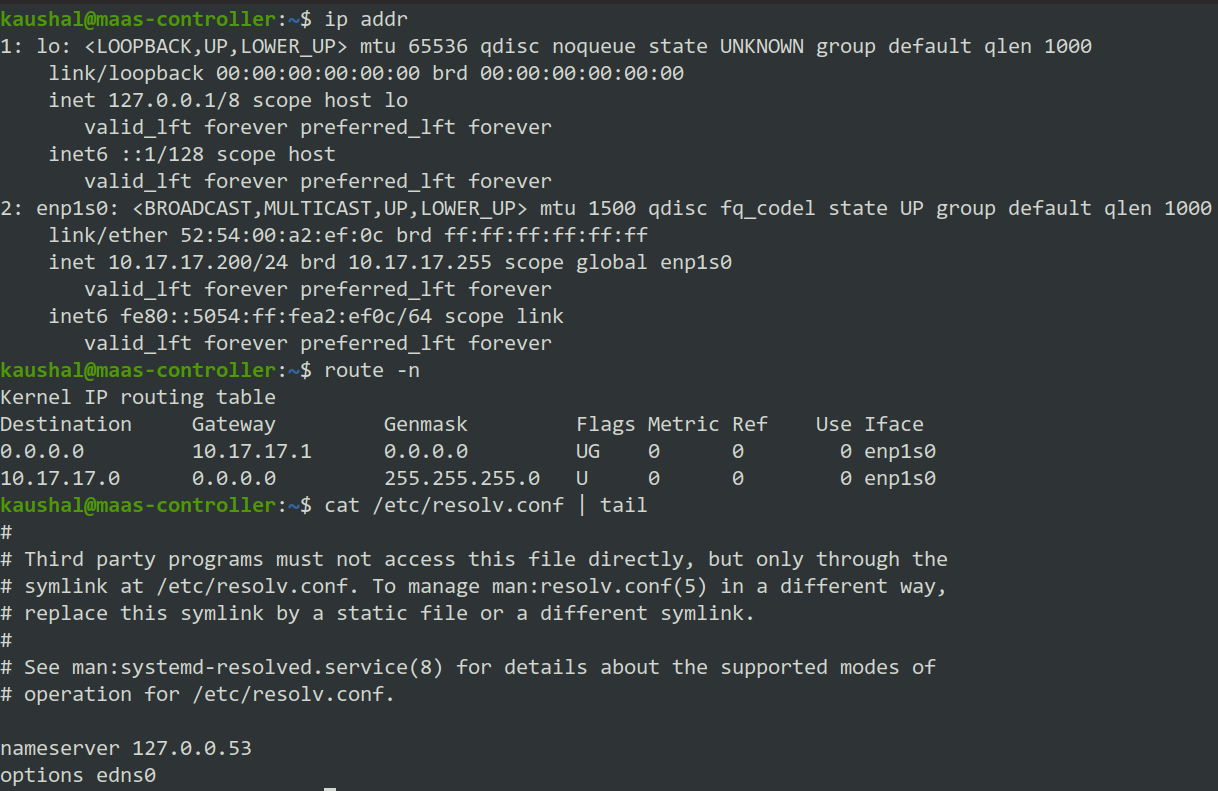
\includegraphics[width=0.7\textwidth]{images/4-4.png}
    \caption{verify internet connectivity}
\end{figure}

Verify the network connectivity by using the following commands:

\begin{itemize}
    \setlength\itemsep{-1em}
    \item[\$] ip addr
    \item[\$] route -n
    \item[\$] cat /run/systemd/resolve/resolv.conf | tail -n 1 
    \item[\$] dig canonical.com
    \item[\$] ping google.com 
\end{itemize}

The results should look similar to Fig. 4.4.

\begin{figure}[!ht]
    \centering
    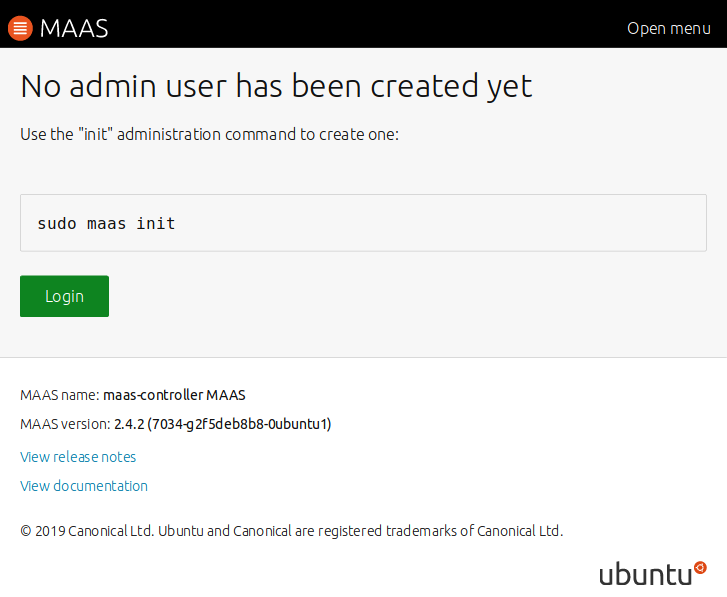
\includegraphics[width=0.5\textwidth]{images/4-5.png}
    \caption{MAAS initial page}
\end{figure}

Verify that the following link works: \url{http://10.17.17.200:5240/}. It will open a MAAS interface which looks something similar to Fig. 4.5. Create a super-user by using the following command: 

\$ sudo maas init

After setting up the maas superuser open the maas webui and login. You will land up on the page similar to Fig. 4-6.

\begin{figure}[!ht]
    \centering
    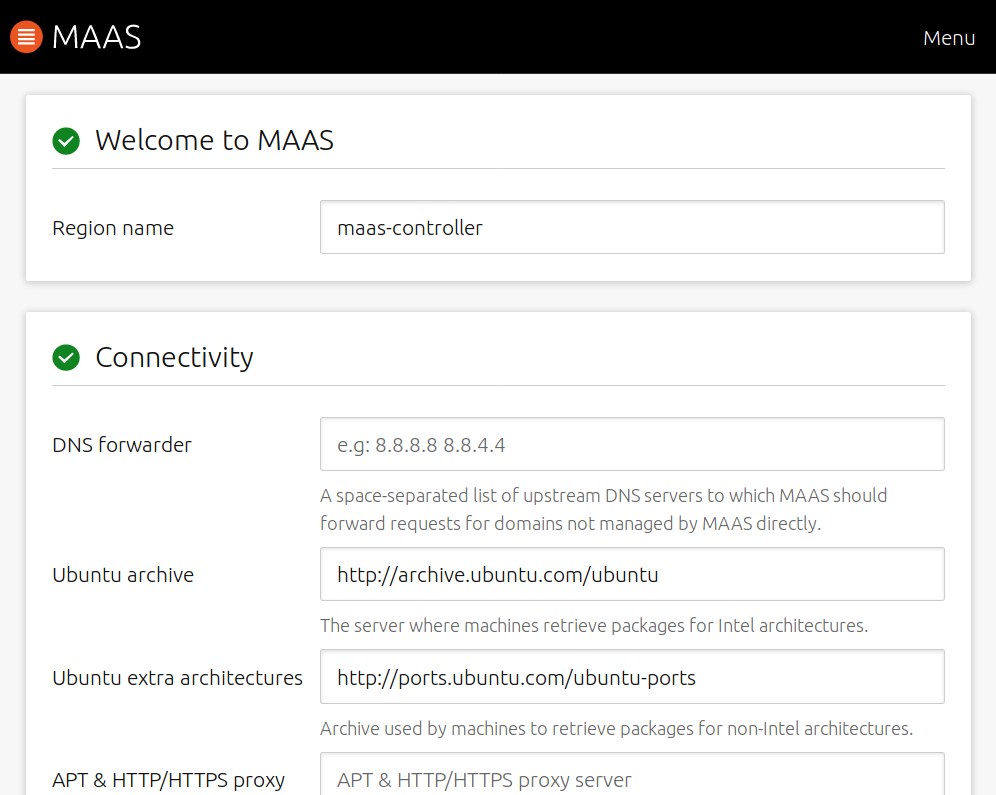
\includegraphics[width=0.5\textwidth]{images/4-6.png}
    \caption{MAAS intro page}
\end{figure}

\section{SSH \& DHCP configuration for MAAS}

Change the default shell of the 'maas' user as shown in the Fig. 4.7.

\begin{figure}[!ht]
    \centering
    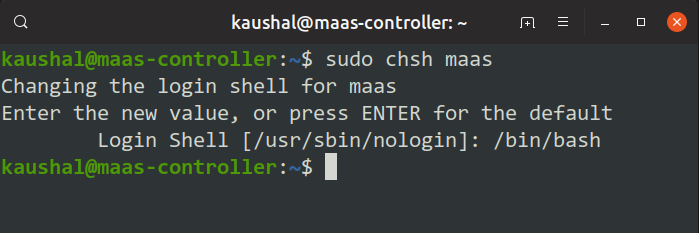
\includegraphics[width=0.5\textwidth]{images/4-7.png}
    \caption{Default shell for maas user}
\end{figure}

Login to the maas user and generate an ssh key and copy the public key to the host for passwordless ssh authentication. That will enable us to open a ssh session at that virtual machine host without being prompted for a password. Verify that you are able to open an ssh session to the host system from the controller without being asked for the password.

\begin{enumerate}
    \setlength\itemsep{-1em}
    \item[\$] sudo su - maas
    \item[\$] ssh-keygen -t rsa
    \item[\$] \url{ssh-copy-id} \url{-i} \url{~/.ssh/id_rsa.pub} \url{kaushal@10.128.0.132}
\end{enumerate}

Verify that maas will be able to control the virtual machines power at the host level. To do that we need to verify that the virsh command is working.

\url{virsh} \url{-c} \url{qemu+ssh://kaushal@10.128.0.132/system} \url{list} \url{--all}

It should list all the virtual machines at the host.

The next thing we need to do is to import the ssh key of maas controller into maas, so that when maas provisions a new node and brings up an image on that node it can inject our ssh key allowing us to remotely access those managed nodes without that we really have no way aside from backdoor and breaking in to access those nodes that we have created.

To do this first create a ssh key by following the above mentioned steps.

Go to the following link: \url{http://10.17.17.200:5240/MAAS/#/intro/user} and upload your ssh key.

\begin{figure}[!ht]
    \centering
    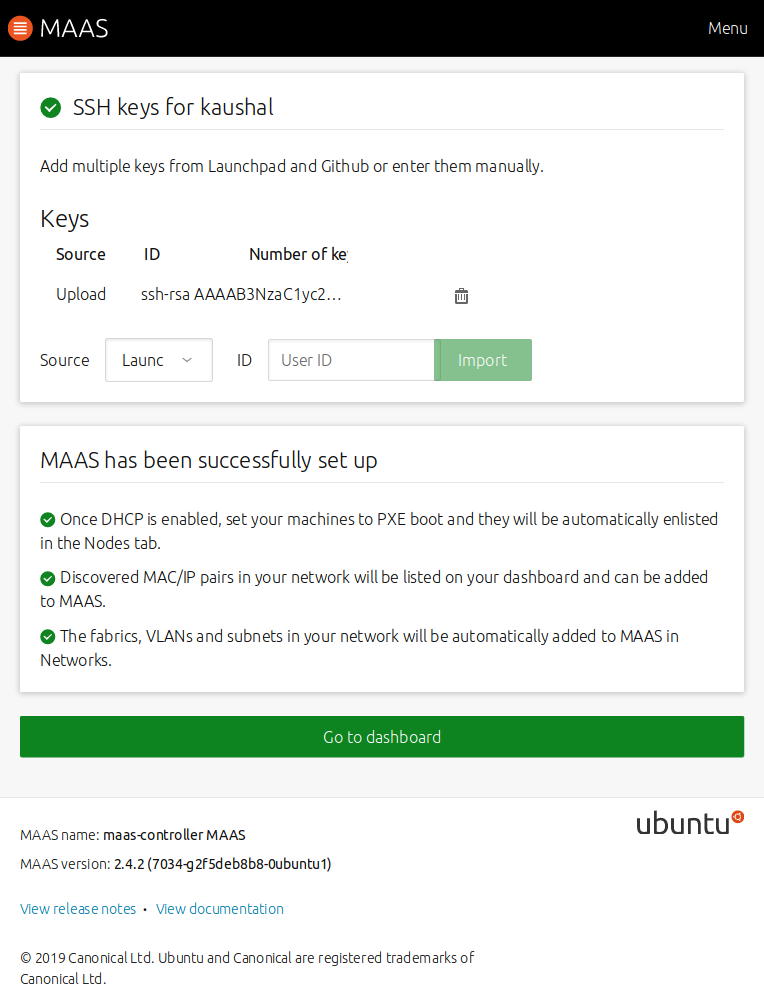
\includegraphics[width=0.5\textwidth]{images/4-8.png}
    \caption{Uploading the ssh key of maas controller}
\end{figure}

Next we need to configure the DHCP configuration for the maas. To enable MAAS-managed DHCP, under the ‘Subnets’ page select the desired fabric and then VLAN.

\subsection{IP Ranges}

During the DHCP configuration we need to configure the IP ranges. IP addresses can be reserved by adding one or more reserved ranges to a subnet configuration. There are two types of ranges that can be defined: reserved range and reserved dynamic range.

\textbf{Reserved range} mode operates differently depending on whether the subnet is \textbf{managed} or \textbf{unmanaged}. In managed (subnet), MAAS will never assign IP addresses inside this range. They can be used for anything (e.g. infrastructure systems, network hardware, or external DHCP). While in unmanaged (subnet), MAAS will only assign IP addresses inside this range.

A \textbf{Reserved dynamic range} is an IP range that MAAS will use for enlisting, commissioning and, if MAAS-managed DHCP is enabled on the node's VLAN during commissioning, deploying. An initial range is created as part of the DHCP enablement process if done with the web UI. For an unmanaged subnet, this range is never used.

To keep things simple we will use the reserved dynamic range mode with managed subnet. By default managed allocation for a subnet is enabled, you can disable it by editing the subnet configuration under the subnet tab and then select the appropriate fabric and then editing the desired subnet.

\begin{figure}[!ht]
    \centering
    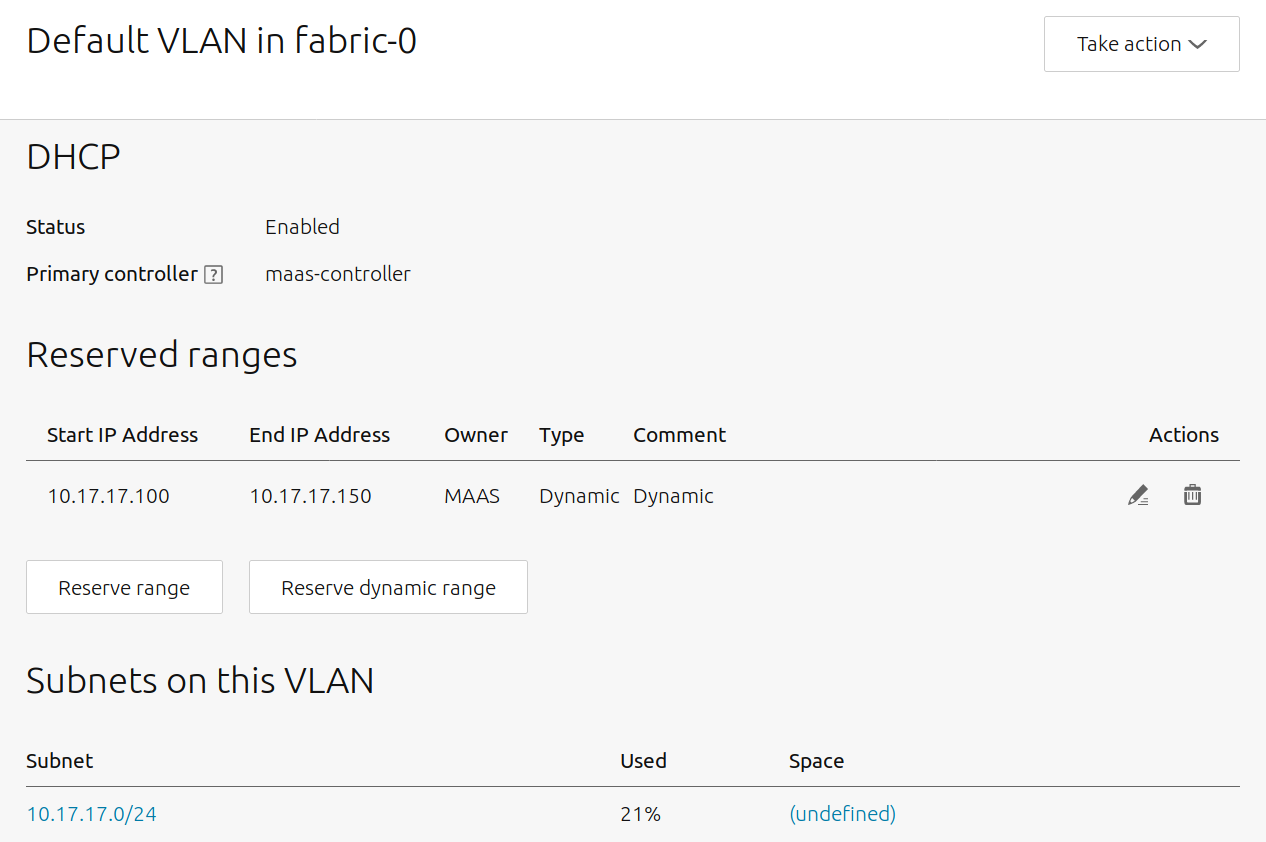
\includegraphics[width=0.5\textwidth]{images/4-9.png}
    \caption{Provide DHCP}
\end{figure}

\begin{figure}[!ht]
    \centering
    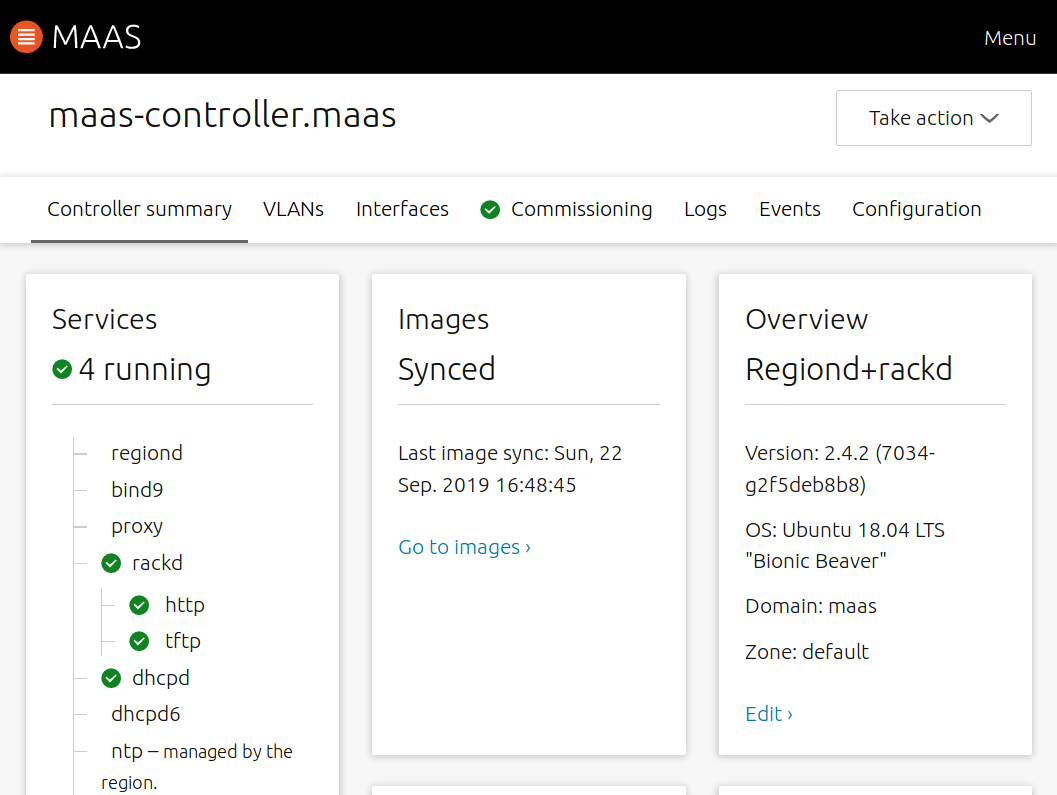
\includegraphics[width=0.5\textwidth]{images/4-10.png}
    \caption{Editing subnet}
\end{figure}

With this our basic configuration of the maas controller is done and in the next chapter we will create some nodes.
